\section{System Model}

\subsection{Task Model}
We consider a task set $\tau$ of ${n}$ sporadic parallel real time tasks,
$\tau = \{\tau_1,\tau_2, ..., \tau_n\}$. A task $\tau_i$ in the task
system generates a potentially infinite number of jobs, each arriving
no less than $T_i$ time units after the previous job and has a constrained
deadline $D_i$ where $D_i \leq T_i$.  Each task $\tau_i \in \tau$ is
considered as a parallel task and is represented as a directed acyclic
graph (DAG) ${G_i}$, the set of DAGs is given as ${G = \{G_1, G_2,
  ..., G_n\}}$. An example DAG is shown in Fig.~\ref{fig:dag}.

\begin{figure}[!h]
  \centering
  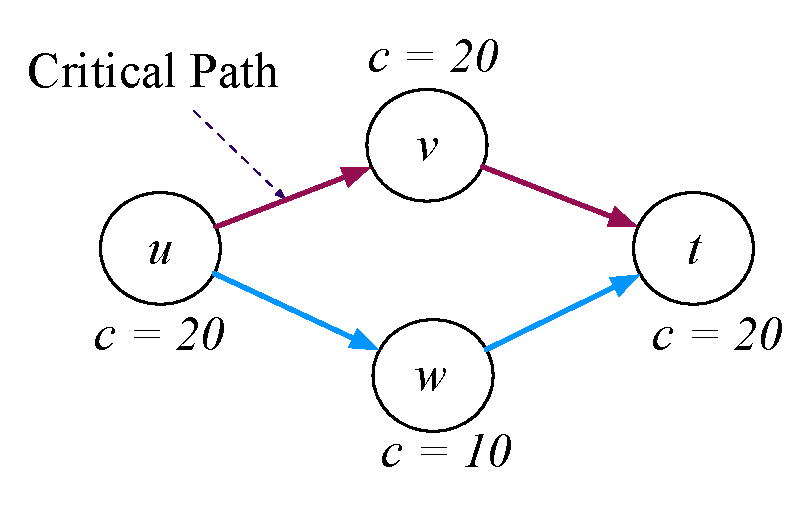
\includegraphics[width=0.4\columnwidth]{dag}
  \caption{An Example of a Parallel Real-time Task}
  \label{fig:dag}
\end{figure}


%%
%% XXX-ct Proposal for streamlining the model
%%
In this work a node ${v_i \in V}$ is represented by a tuple
${v_i = \langle A, c_i, m_i \rangle }$ where ${A}$ is the code segment
the thread will execute, ${c_i}$ is the WCET function for ${m_i}$
threads associated with each node. \revise{transition sentence
  describing ${c_i(m_i)}$} This is compatible with the previous model
\revise{citation needed} where ${v_i = <A, c_i(1), 1>}$. 

\revise{A node $v_i^j \in V_i$ is expressed as a double <$cs_i^j$, $c_i^j$>, where $cs_i^j$ denotes the code segment executed by a thread and $c_i^j$ denotes the worst-case execution time of the thread execution.}
Each node ${v \in V_i}$ of a DAG ${G_i = (V_i, E_i)}$ represents the
execution of a thread and an ${e \in E_i}$ edge represents a
dependency between two nodes. A dependency between two nodes indicates
that a node is ready to execute only upon the completion of all its
predecessor nodes. We consider a source as a node with no incoming
arcs and a sink as node with no outgoing arcs. For the sake of
simplicity, we assume a task has only one source and sink node. In
practice, this not hard to achieve as a source and sink can be added
to the task with $0$ execution and not change the task dependencies.

%Nodes of a task have an associated worst-case execution time. 
\revise{For a node $v_i^j$, we define $parent(v_i^j)$ and $child(v_i^j)$ as a set of parent nodes of $v_i^j$ and a set of child nodes of $v_i^j$, respectively. we define $pre(v_i^j)$ and $succ(v_i^j)$ as a set of all predecessors of $v_i^j$ and a set of all successors of $v_i^j$, respectively.}
For any given task, we define a \textit{critical path} $\lambda_i$ of a 
task $\tau_i$ as the longest execution time path that starts from
source and ends at the sink. \textit{Critical path length} ($L_i$) is
defined as the sum of execution times of all nodes along the critical
path $\lambda_i$ of task $\tau_i$.  Workload $C_i$ of
a task $\tau_i$ is defined as the sum of worst-case execution time of
all nodes in the DAG task. 


\subsection{Federated Scheduler}
For a task set $\tau$ , the federated scheduling algorithm works as
follows. We first divide the task sets into two disjoint sets
$\tau_{high}$  and $\tau_{low}$. $\tau_{high}$ contains all tasks with
high utilization (i.e. $u_i > 1$) and $\tau_{low}$ contains all
remaining low utilization tasks. Each task in $\tau_{high}$ is
assigned $m_i$ dedicated cores (no other task is executed on these
cores), where: \begin{equation}\label{eq:m} m_i = \left\lceil \frac{C_i - L_i}{D_i - L_i}
\right\rceil \end{equation}

We use $m_{high} = \sum_{\tau_i \in \tau_{high}} m_i$ to denote the total
number of cores assigned to high-utilization tasks. We assign
the remaining cores to all low-utilization tasks $\tau_{low}$, denoted
as ${m_{low} = m - m_{high}}$. The federated scheduling algorithm admits
the task set ${\tau}$, if $m_{low}$ is non-negative and all tasks in
$\tau_{low}$ are schedulable sequentially.  

After a valid core allocation, runtime scheduling proceeds as
follows. Any greedy (work-conserving) parallel scheduler can be used
to schedule a high-utilization task $\tau_i \in \tau_{high}$ on its
assigned $m_i$ cores. Informally, a greedy scheduler is one that never
keeps a core idle if some node is ready to execute. 

All low-utilization tasks are treated and executed as though they are
sequential tasks and any multiprocessor scheduling algorithm (such as
partitioned EDF, or various rate-monotonic schedulers) can be used to
schedule all the low-utilization tasks on the allocated $m_{low}$
cores. We can safely treat low-utilization tasks as sequential tasks
since $C_i \le D_i$ and parallel execution is not required to meet their
deadlines. 

\subsection{Processing Model}

In this work, for each core, we assume a dedicated direct mapped
instruction cache. We assume a time-compositional architecture\addcite,
where memory and execution demand are separable. Copying a block of 
main memory to cache memory requires ${\mathbb{B}}$ cycles, commonly
referred to as the the block reload time (BRT). If multiple cores share
the same processing platform their cache contents do not interfere with
one another. The impact of a shared cache between cores is not considered.


\section{Proposed Changes to the Directed Acyclic Graph Model of Parallel Systems}

For a DAG ${G = (V, E)}$ representing a parallel task, each node ${v_i \in V}$ represents
the release, execution, and termination of a single thread within one task 
\addcite. In the existing model, the only relationship between thread releases and the executable object they execute is the worst-case execution time of the node. Two nodes ${v_i, v_j \in V}$ may represent two threads executing the same object (possibly on different processors).

\begin{figure}
  \centering
  \begin{subfigure}[b]{0.4\textwidth}{
      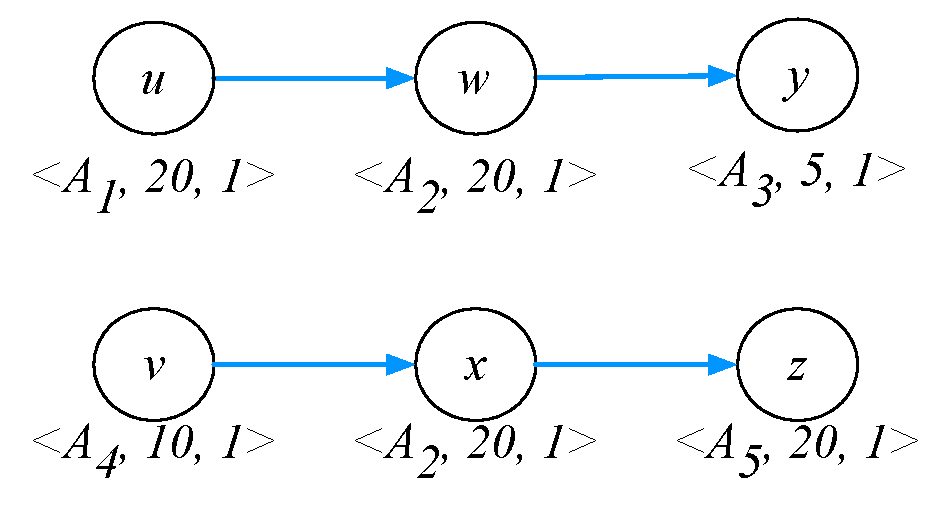
\includegraphics[width=\textwidth]{beforeCollapse}
      \caption{Before Collapse}
      \label{fig:before-collapse}
    }
  \end{subfigure} \quad
  \begin{subfigure}[b]{0.4\textwidth}{
      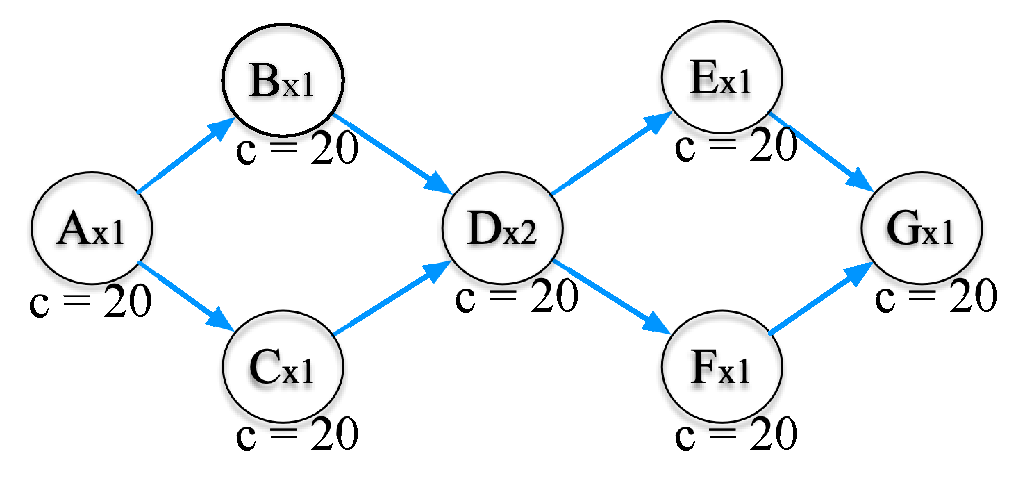
\includegraphics[width=\textwidth]{afterCollapse}
      \caption{After Collapse}
      \label{fig:after-collapse}
    }
  \end{subfigure}
  \caption{DAG Node Change from Thread to Code Segment}
  \label{fig:dag-change}
\end{figure}

To take advantage of instruction cache reuse, we propose a simple modification to the DAG
model. Where possible, distinct nodes that represent the execution of
the same object are collapsed into a single node. To accommodate collapse,
nodes are identified by their executable object, and a new attribute is added to every node
indicating the number of threads which will be executed over the object.

\revise{Given the new model to represent a node, two nodes $v_i^j$, $v_i^k$ with the same code segments (i.e., $cs_i^j = cs_i^k$ and $c_i^j = c_i^k$) are collapsed into one node $v_i^h$, where $v_i^h = <cs_i^j, c_i^j, \max{\eta_i^j, \eta_i^k}+1>$.  To ensure dependencies of the DAG are not violated, we replace the edges that start from $v_i^j$ and $v_i^k$  to start from $v_i^h$, i.e., the child nodes of $v_i^h$ are given as a union of the child nodes of $v_i^j$ and $v_i^k$, $child(v_i^h) = child(v_i^j) \cup child(v_i^k)$. Similarly, parent nodes of $v_i^h$ are given as a union of the parent nodes of $v_i^j$ and $v_i^k$, i.e., $parent(v_i^h) = parent(v_i^j) \cup parent(v_i^k)$.}

Figure~\ref{fig:dag-change} illustrates the proposed change. Nodes in
Figure~\ref{fig:before-collapse} are labeled with the code segment
they are associated with. Two nodes of ${B}$ are collapsed in
Figure~\ref{fig:after-collapse}, where each node is attributed with
the number of threads executed over the code segment.

A goal of this work is to bring the inter-thread cache benefit \addcite to parallel DAG tasks. 

%% ct - commented out because splitting a code segment into multiple code segments may introduce loops in the DAG. 
%%		For example, if a loop is too big and cannot fit into a cache block then we it will be split across multiple segments which will introduce a DAG.
%%
%%A goal of this work is to bring the inter-thread cache benefit \addcite to parallel DAG tasks. As a first-step, two requirements are placed on nodes of the graph.
%%\begin{description}
%%\item[R1] All executable objects must fit entirely within the cache.
%%\item[R2] No two instructions of an executable object may evict one another.
%%\end{description}
%%
%%Requirements R1 and R2 may be met for any executable object by repeatedly dividing
%%the object source that result in objects larger than the cache into separate code segments, carefully recompiling those code segments to maximize cache use, and replacing the original node with a serial set of nodes.
%%\\
%%\\
%%\emph{ct-3 A figure is needed to illustrate the transformation from one over-sized node, to multiple correctly sized nodes}
%%\\

In the established model \addcite, each node ${v_i^j \in V_i}$ is characterized
with a single worst case execution time for a single thread. We
propose that each node's WCET is characterized by a function
${c_i^j(\eta_i^j)}$ where ${\eta_i^j}$ is the number of threads that will execute the
node ${v_i^j}$ on the same core serially (one after another) with no
other thread executing a different object on the core in between executions.

%%Given a timing-compositional architecture with the restrictions \textbf{R1} and \textbf{R2},
Given a timing-compositional architecture
${c_i(n)}$ can be expressed for any node in terms of the memory demand of all instructions
of ${v_j \in V_i}$ into the cache ${\gamma_j}$ and the worst-case execution demand
to execute the node assuming all instructions of ${v_j}$ have
been cached ${\iota_j}$. Equation~\ref{eq:c_i} is an expression for
${c_i(n)}$. 
 
\begin{equation}
  \label{eq:c_i}
  c_i(n) = \begin{cases}
    0, & n \le 0 \\
    \gamma_j + \iota_j \cdot n, & n > 0
  \end{cases}
\end{equation}

For a node ${v_i \in V_j}$, the upper bound of memory demand of the node is denoted ${\gamma_i}$. It is the number of cycles required to load all blocks of the node. The complete set of blocks of the node are equivalent to the evicting cache blocks (ECBs)\addcite [Tan \& Mooney] of the object. Thus, the memory demand is the product of the BRT and count of ECBs of the node ${\textsc{ecb}_i}$ found in Equation~\ref{eq:mem-demand}.

\begin{equation}{\label{eq:mem-demand}}
    \gamma_i = \mathbb{B} \cdot \textsc{ecb}_i
\end{equation}

The execution demand ${\iota_i}$ for a node ${v_i^j \in V_i}$ is the worst case execution time of a single thread given all instructions are present in the cache. Any suitable WCET calculation method {\addcite} may be used to calculate the value.

%%\section{Problem Formulation}
